% Template for ICIP-2019 paper; to be used with:
%          spconf.sty  - ICASSP/ICIP LaTeX style file, and
%          IEEEbib.bst - IEEE bibliography style file.
% --------------------------------------------------------------------------
\documentclass{article}
\usepackage{spconf,amsmath,graphicx}

% Example definitions.
% --------------------
\def\x{{\mathbf x}}
\def\L{{\cal L}}

% Title.
% ------
\title{Face Recognition using HOG Feature and SVM}
%
% Single address.
% ---------------
\name{Srushanth Baride}
\address{University of Nottingham}
%
%
\begin{document}
%\ninept
%
\maketitle
%
\begin{abstract}
    There are many advancements in the technology solving very difficult problems of the society. One of the alleged controversial technologies in the times is Face Recognition systems. These systems are majorly used in the banking and security sectors. There are numerous algorithms developed in the past few decades to perform Face Recognition like LBPH (Local Binary Patterns Histograms), Fisherfaces, Eigenfaces, SURF (Speed Up Robust Features) and HOG (Histogram of Oriented Gradients). HOG is used in this paper for the purpose of feature extraction. The PCA an important feature method in Eigen faces method is today an important brainwave for almost all the face recognition algorithms unfolded into new and better programming methods \cite{1article}.
\end{abstract}
%
\begin{keywords}
LBPH, Fisherfaces, Eigenfaces, SURF, HOG
\end{keywords}
%
\section{Introduction}
\label{sec:intro}

In this paper, an intelligent Face Recognition System is developed using MATLAB. The same solution can also be used for the purpose of object detection and object tracking systems. There are many individual developers and multi national companies are who are working to develop and improve the Face Recognition technology. This technology is being used in many security applications like banking, social indexing, Access control, Image Database Investigation, General identity verification, Surveillance, etc \cite{2article}.

The first and foremost tasks performed in this project is to process the data beforehand. In this scenario, the image size is resized to be compatible with both HOG feature extractor and Deep Learning alexnet.

The dataset is split into training and testing set and the pictures are sent to the HOG feature extractor. Once the features are extracted, the data is sent through the SVM (Support Vector Machine) classifier to train the model to detect different persons.

\section{HOG (Histogram of Oriented Gradients)}
\label{sec:format}

HOG (Histogram of Oriented Features) \cite{unknown-author-2022} is a feature descriptor mostly used in the field of Computer Vision for Object Detection, Object Tracking and Facial Recognition applications.

Robert K. McConnell of Wayland Research Inc. first described the concept behind HOG without using the term HOG in a patent application in 1986 \cite{mcconnell1986method}.

HOG descriptors may be used for object recognition by providing them as features to a machine learning algorithm. Dalal and Triggs used HOG descriptors as features in a support vector machine (SVM);\cite{1467360} however, HOG descriptors are not tied to a specific machine learning algorithm.

To make the HOG feature descriptor, we need to calculate the respective horizontal and vertical gradients to actually provide the histogram that can be used in the algorithm. This can be done by simply filtering the image through these kernels \cite{mittal-2021}.

\begin{equation}
    \begin{bmatrix}
    -1 & 0 & 1
    \end{bmatrix}
\end{equation}

\begin{equation}
    \begin{bmatrix}
    -1\\
    0\\
    1
    \end{bmatrix}
\end{equation}
Kernels like these are often used in image classification mainly in convolutional neural networks in order to find the edges and important points in a particular image.

The magnitude and direction gradients from an image can be calculated using the below equations.

\begin{equation}
    Gradient\ Magnitude = \sqrt{(Gradient_X)^2+(Gradient_Y)^2}
\end{equation}

\begin{equation}
    Gradient\ Direction = \tan^{-1}(Gradient_X/Gradient_Y)
\end{equation}

Feature descriptors will allow for a concise and succinct representation of particular patches of the images. A 8x8 cell can simply be explained using 128 numbers (8x8x2 where the last 2 are from the gradient magnitude and directional values). By further converting these numbers to calculate histograms, we allow for an image patch that is much more robust to noise and more compact.

\begin{figure}
    \centering
    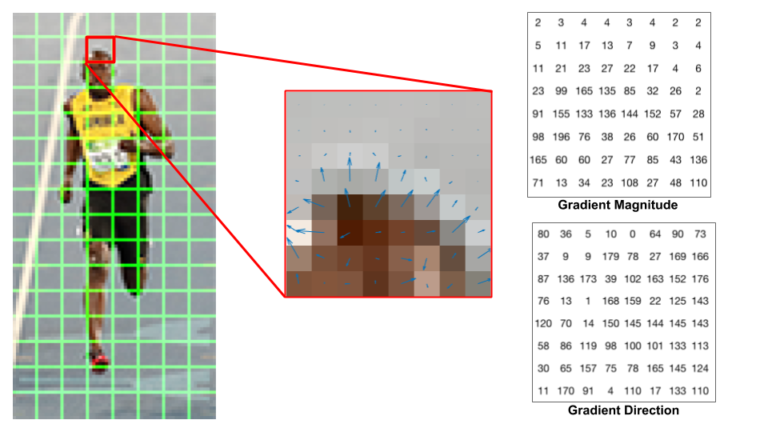
\includegraphics[width=9cm]{Images/1_HhsKGuHj2zhr2ny9MyvryA.png}
    \caption{Center : The RGB patch and gradients represented using arrows. Right : The gradients in the same patch represented as numbers\cite{mallick-2021}}
\end{figure}

A bin is selected depending on the direction chosen, and the value that is subsequently placed inside of the bin is dependent on the magnitude. If a pixel is halfway between two bins, then it splits up the magnitudes accordingly depending on their distance away from each respective bin. After performing this process, a histogram can be formed, and the bins that have the most weight can easily be seen.


\section{SVM (Support Vector Machines)}


SVM is a supervised Machine Learning algorithm i.e., used for both classification and regression problems. The SVM algorithm separates the classes using lines or hyperplanes. The SVM takes data or features as input and outputs a line or a plane which separates the different classes in the data.

SVM finds the closest data points separating the two classes, these points are called as support vectors and draws a line separating then such as the distance between the points are maximum.

\begin{figure}
    \centering
    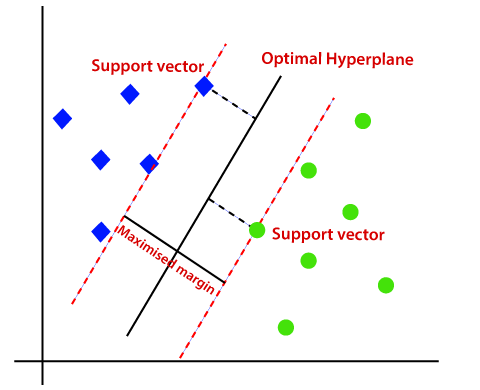
\includegraphics[width=9cm]{Images/Picture2.png}
    \caption{Optimal Hyperplane using the SVM algorithm\cite{pupale-2022}}
    \label{fig:galaxy}
\end{figure}


\section{Methodology and Setup }
\label{sec:pagestyle}

The paper title (on the first page) should begin 1.38 inches (35 mm) from the
top edge of the page, centered, completely capitalized, and in Times 14-point,
boldface type.  The authors' name(s) and affiliation(s) appear below the title
in capital and lower case letters.  Papers with multiple authors and
affiliations may require two or more lines for this information. Please note
that papers should not be submitted blind; include the authors' names on the
PDF.

\begin{enumerate}
    \itemsep0em 
    \item Pre-process the images
        \begin{enumerate}
            \item Define destination image size and image type
            \item Load the complete raw data i.e., images
            \item Load the image from the raw data
            \item resize the image and save to the destination directory
            \item Repeat the steps from (c) for all the remaining images
        \end{enumerate}
    \item Load the complete raw data i.e., images from the processed directory
    \item Split the data into train and test dataset's
    \item Use Feature extractor to extract the features the loaded data
        \begin{enumerate}
            \item Extract HOG features from all the images
        \end{enumerate}
    \item Use Machine Learning algorithm to classify the classes from the dataset
        \begin{enumerate}
            \item SVM (Support Vector Machines) is used to classify the classes from HOG features
        \end{enumerate}
    \item Test the accuracy of the model on test dataset
    \item Save the model
    \item Infer the data using a different or real-time streaming data
\end{enumerate}

\section{TYPE-STYLE AND FONTS}
\label{sec:typestyle}

To achieve the best rendering both in printed proceedings and electronic proceedings, we
strongly encourage you to use Times-Roman font.  In addition, this will give
the proceedings a more uniform look.  Use a font that is no smaller than nine
point type throughout the paper, including figure captions.

In nine point type font, capital letters are 2 mm high.  {\bf If you use the
smallest point size, there should be no more than 3.2 lines/cm (8 lines/inch)
vertically.}  This is a minimum spacing; 2.75 lines/cm (7 lines/inch) will make
the paper much more readable.  Larger type sizes require correspondingly larger
vertical spacing.  Please do not double-space your paper.  TrueType or
Postscript Type 1 fonts are preferred.

The first paragraph in each section should not be indented, but all the
following paragraphs within the section should be indented as these paragraphs
demonstrate.

\section{MAJOR HEADINGS}
\label{sec:majhead}

Major headings, for example, "1. Introduction", should appear in all capital
letters, bold face if possible, centered in the column, with one blank line
before, and one blank line after. Use a period (".") after the heading number,
not a colon.

\subsection{Subheadings}
\label{ssec:subhead}

Subheadings should appear in lower case (initial word capitalized) in
boldface.  They should start at the left margin on a separate line.
 
\subsubsection{Sub-subheadings}
\label{sssec:subsubhead}

Sub-subheadings, as in this paragraph, are discouraged. However, if you
must use them, they should appear in lower case (initial word
capitalized) and start at the left margin on a separate line, with paragraph
text beginning on the following line.  They should be in italics.

\section{PAGE NUMBERING}
\label{sec:page}

Please do {\bf not} paginate your paper.  Page numbers, session numbers, and
conference identification will be inserted when the paper is included in the
proceedings.

\section{ILLUSTRATIONS, GRAPHS, AND PHOTOGRAPHS}
\label{sec:illust}

Illustrations must appear within the designated margins.  They may span the two
columns.  If possible, position illustrations at the top of columns, rather
than in the middle or at the bottom.  Caption and number every illustration.
All halftone illustrations must be clear black and white prints.  Colors may be
used, but they should be selected so as to be readable when printed on a
black-only printer.

Since there are many ways, often incompatible, of including images (e.g., with
experimental results) in a LaTeX document, below is an example of how to do
this.

\section{FOOTNOTES}
\label{sec:foot}

Use footnotes sparingly (or not at all!) and place them at the bottom of the
column on the page on which they are referenced. Use Times 9-point type,
single-spaced. To help your readers, avoid using footnotes altogether and
include necessary peripheral observations in the text (within parentheses, if
you prefer, as in this sentence).

% To start a new column (but not a new page) and help balance the last-page
% column length use \vfill\pagebreak.
% -------------------------------------------------------------------------
%\vfill
%\pagebreak


\bibliography{bibliography}
\bibliographystyle{IEEEtran}

\end{document}
